%%=============================================================================
%% Methodologie
%%=============================================================================

\chapter{\IfLanguageName{dutch}{Methodologie}{Methodology}}%
\label{ch:methodologie}

%% TODO: In dit hoofstuk geef je een korte toelichting over hoe je te werk bent
%% gegaan. Verdeel je onderzoek in grote fasen, en licht in elke fase toe wat
%% de doelstelling was, welke deliverables daar uit gekomen zijn, en welke
%% onderzoeksmethoden je daarbij toegepast hebt. Verantwoord waarom je
%% op deze manier te werk gegaan bent.
%% 
%% Voorbeelden van zulke fasen zijn: literatuurstudie, opstellen van een
%% requirements-analyse, opstellen long-list (bij vergelijkende studie),
%% selectie van geschikte tools (bij vergelijkende studie, "short-list"),
%% opzetten testopstelling/PoC, uitvoeren testen en verzamelen
%% van resultaten, analyse van resultaten, ...
%%
%% !!!!! LET OP !!!!!
%%
%% Het is uitdrukkelijk NIET de bedoeling dat je het grootste deel van de corpus
%% van je bachelorproef in dit hoofstuk verwerkt! Dit hoofdstuk is eerder een
%% kort overzicht van je plan van aanpak.
%%
%% Maak voor elke fase (behalve het literatuuronderzoek) een NIEUW HOOFDSTUK aan
%% en geef het een gepaste titel.
\section{Methodologie}

\subsection{Data Verzameling en Verwerking}
De eerste fase van het onderzoeksproces bij ArcelorMittal betreft de verzameling en verwerking van omvangrijke datasets die dagelijkse productie- en energieverbruiksgegevens bevatten. Deze gegevens zijn afkomstig uit de operationele databases van het bedrijf, die automatisch de belangrijke parameters registreren die nodig zijn voor de analyse van het energieverbruik in de staalproductieprocessen.

De verzamelde dataset bevat gedetailleerde metingen zoals de datum, gemiddelde breedte en dikte van de geproduceerde slabs, het energieverbruik van de ovens zowel tijdens de productie als in rusttoestand, en het totale gewicht van de geproduceerde slabs per oven. Deze parameters zijn essentieel om inzicht te krijgen in de energie-efficiëntie van de productiefaciliteiten en om correlaties te identificeren tussen de operationele variabelen en het energieverbruik.

Een zorgvuldige data voorbereiding volgt op de verzameling om de kwaliteit en consistentie van de dataset te waarborgen. Dit proces omvat het controleren van de data op ontbrekende waarden, het corrigeren van foutieve of abnormale gegevensinvoer, en het normaliseren van de numerieke gegevens om uniformiteit in schaal en verdeling te garanderen. Deze stappen zijn cruciaal om ervoor te zorgen dat de machine learning modellen betrouwbare en valide resultaten opleveren.

De normalisatieprocedure maakt gebruik van technieken zoals min-max scaling, die elke feature schaalt binnen een gedefinieerd bereik, meestal 0 tot 1. Dit helpt bij het verminderen van mogelijke vertekeningen die kunnen ontstaan door variabelen die op verschillende schalen opereren, waardoor de impact van grotere numerieke waarden wordt geminimaliseerd en de training van het model efficiënter verloopt.

Deze initiële stappen van dataverzameling en -verwerking zijn fundamenteel voor het succes van het onderzoek, aangezien de kwaliteit en precisie van de inputdata direct invloed hebben op de nauwkeurigheid van de energieverbruiksvoorspellingen die uit het model voortvloeien.

\subsection{Feature Engineering}
Een cruciale stap in de voorbereiding van de data voor machine learning is feature engineering, waarbij relevante kenmerken worden geselecteerd en getransformeerd om de voorspellingskracht van het model te optimaliseren. In het onderzoek bij ArcelorMittal is deze stap bijzonder belangrijk vanwege de complexe aard van de productieprocessen en de diverse factoren die het energieverbruik beïnvloeden.

\begin{figure}[h!]
    \centering
    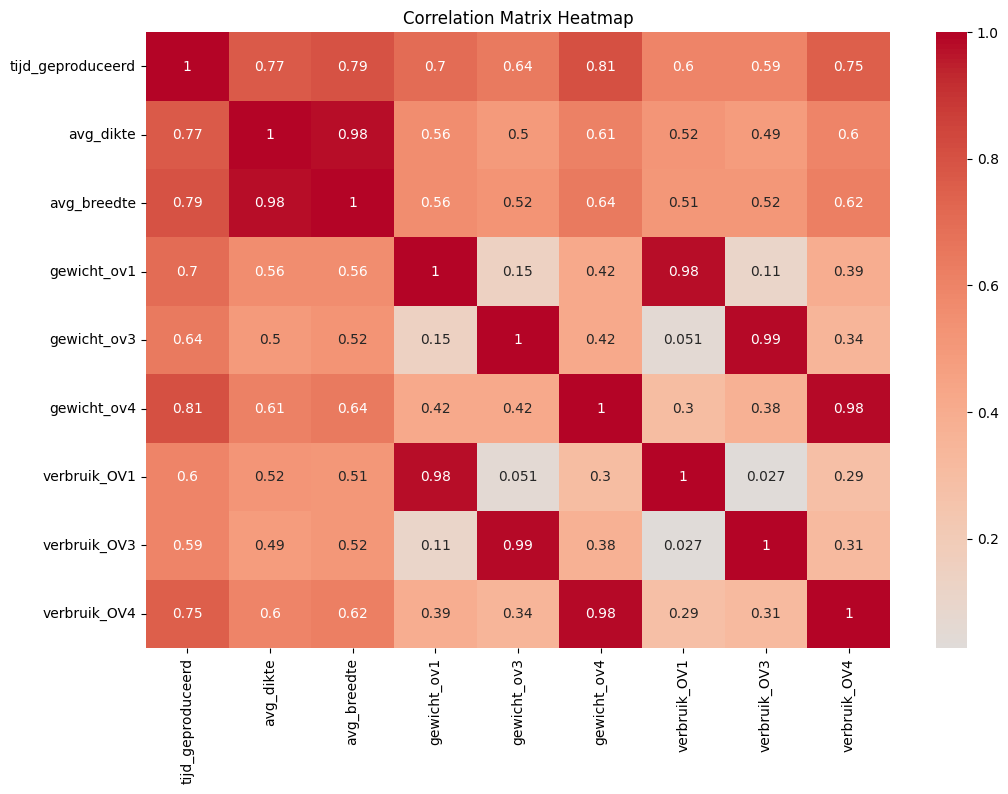
\includegraphics[width=\textwidth]{graphics/FeatureMap.png}
    \caption{Feature map die de geselecteerde en getransformeerde kenmerken toont voor het optimaliseren van het voorspellingsmodel.}
    \label{fig:FeatureMap}
\end{figure}

\subsubsection{Selectie van Kenmerken}
De kenmerken die gekozen zijn voor het LSTM-model omvatten de tijd geproduceerd, de gemiddelde dikte en breedte van de slabs, en het gewicht van de slabs per oven. Deze kenmerken zijn geselecteerd op basis van hun vermoedelijke invloed op het energieverbruik. Enerzijds reflecteren de productietijd en de afmetingen van de slabs de operationele intensiteit en efficiëntie, terwijl het gewicht van de slabs kan duiden op de belasting van de ovens.

\subsubsection{Transformatie en Normalisatie}
De geselecteerde kenmerken ondergaan vervolgens een reeks transformaties om ze geschikter te maken voor modeltraining. Normalisatie is een standaardpraktijk, die ervoor zorgt dat alle kenmerken bijdragen op een evenwichtige manier zonder dat enkele kenmerken onevenredig veel gewicht krijgen vanwege hun schaal. MinMaxScaler is een veelgebruikte techniek die elk kenmerk schaalt naar een bereik tussen 0 en 1, waardoor de impact van uitschieters wordt geminimaliseerd en de algehele modelprestaties worden verbeterd.

\subsubsection{Het Creëren van Trainingsets}
Na de normalisatie worden de kenmerken gecombineerd in trainingsets die gebruikt worden om het model te voeden. Elk record in de trainingset bevat een vector van kenmerken die de input vormt voor het LSTM-netwerk, samen met het werkelijke energieverbruik van de ovens, dat als target dient. Door de samenhang tussen deze kenmerken en het energieverbruik te analyseren, kan het model complexe patronen leren die niet direct zichtbaar zijn uit de ruwe data alleen.

Deze geavanceerde feature engineering benadert niet alleen de technische aspecten van het bouwen van een voorspellend model, maar richt zich ook op het begrijpen van de onderliggende processen die het energieverbruik binnen de staalproductie beïnvloeden. Deze diepgaande analyse helpt bij het verfijnen van het model om nauwkeurigere en betrouwbare voorspellingen te genereren.

\subsection{Modelselectie en Training}

\subsubsection{Modelselectie}
Bij het kiezen van het juiste model voor energievoorspelling bij ArcelorMittal, is een reeks voorlopige tests uitgevoerd met verschillende machine learning-modellen. Initieel zijn basisversies van algoritmen zoals lineaire regressie, beslisbomen, en eenvoudige neurale netwerken uitgeprobeerd om een benchmark van prestaties te vestigen. Deze initiële fase hielp bij het identificeren van de beperkingen van minder complexe modellen in het omgaan met de complexiteit en de temporele aard van de dataset.

De keuze viel uiteindelijk op een Long Short-Term Memory (LSTM) netwerk vanwege zijn vermogen om lange termijn afhankelijkheden in tijdreeksdata te leren, wat cruciaal is voor het accuraat voorspellen van energieverbruik gebaseerd op historische productiegegevens. LSTM-netwerken zijn specifiek ontworpen om problemen van verdwijnende en exploderende gradiënten te overkomen, die vaak voorkomen bij standaard recurrente neurale netwerken (RNNs).

\begin{figure}[h!]
    \centering
    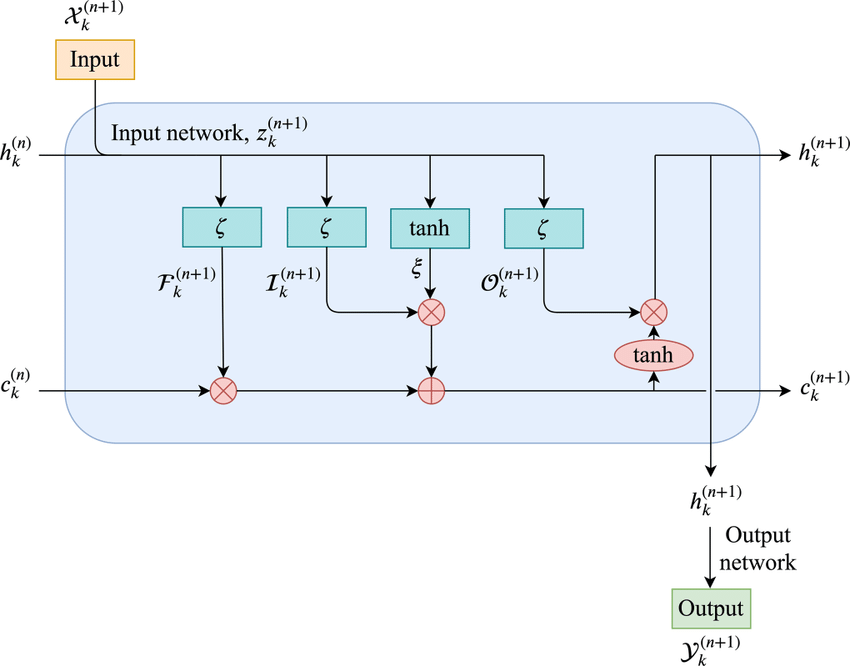
\includegraphics[width=\textwidth]{graphics/LSTMSchematic.png}
    \caption{Schematische voorstelling van een typisch LSTM model.}
    \label{fig:LSTMSchematic}
\end{figure}

\subsubsection{Modelarchitectuur}
De gekozen LSTM-modelarchitectuur is gebaseerd op inzichten uit de literatuur, waaronder de studie van \textcite{Wang_2020}, die de voordelen van een gelaagde LSTM-benadering voor energievoorspelling benadrukt. Het model bestaat uit meerdere lagen die diepte en complexiteit in de verwerking toevoegen, wat resulteert in een robuustere leerervaring:
\begin{itemize}
    \item Eerste LSTM-laag: Deze laag bevat 256 units en retourneert sequenties. Dit betekent dat elke unit output levert voor elke tijdstap, wat bijdraagt aan het behoud van temporele informatie door het netwerk.
    \item Tweede LSTM-laag: Met 128 units, ook retournerend sequenties, draagt deze laag verder bij aan het analyseren van de informatie over langere tijdspannes.
    \item Derde LSTM-laag: Deze laag met 64 units retourneert geen sequenties maar enkel de laatste output, die dient als samenvatting van de geleerde informatie uit de voorgaande lagen.
    \item Dense Output Laag: Een Dense laag wordt gebruikt om de uiteindelijke voorspelling te doen, gebaseerd op de verwerkte informatie uit de LSTM-lagen.
\end{itemize}

\subsubsection{Modeltraining}
Het trainen van het LSTM-model vereist zorgvuldige configuratie van parameters en instellingen om de beste resultaten te bereiken. De volgende stappen, gebaseerd op \textcite{Wang_2020}, worden genomen tijdens het trainingsproces:
\begin{itemize}
    \item Sequence Length: Bepaald op 64 tijdstappen, wat het beste evenwicht biedt tussen tijdsresolutie en rekencomplexiteit.
    \item Optimizer: De Adam optimizer is gekozen voor zijn efficiënte afhandeling van grote datasets en zijn adaptieve leersnelheidseigenschappen.
    \item Loss Functie: Mean Squared Error (MSE) wordt gebruikt als verliesfunctie, om de gemiddelde kwadratische afwijking tussen de voorspelde en werkelijke energieverbruiken te minimaliseren.
    \item Early Stopping: Om overfitting te voorkomen, is een early stopping mechanisme geïmplementeerd, dat de training stopt zodra de validatieloss begint te stijgen, ondanks verdere training.
\end{itemize}

Door deze methodische benadering van modelselectie en -training, gebaseerd op de bevindingen van \textcite{Wang_2020}, is het mogelijk een model te ontwikkelen dat zowel nauwkeurig als betrouwbaar is in het voorspellen van energieverbruik, terwijl het ook robuust genoeg is om te generaliseren naar nieuwe, ongeziene data.

\subsection{Model Evaluatie}

\subsubsection{Evaluatiestrategie}
Na de training van het LSTM-model is het cruciaal om de prestaties ervan grondig te evalueren om te verzekeren dat het betrouwbare en nauwkeurige voorspellingen levert. Deze evaluatie gebeurt door het model te testen met een aparte dataset, die niet is gebruikt tijdens de training. Dit zorgt voor een onpartijdige beoordeling van het model.

\subsubsection{Prestatie-indicatoren}
Voor de evaluatie van het model worden verschillende statistische maten gebruikt:
\begin{itemize}
    \item \textbf{Root Mean Square Error (RMSE):} Deze metriek meet de gemiddelde grootte van de fouten in de voorspellingen van het model, waarbij hogere waarden duiden op grotere fouten. Een lagere RMSE-waarde duidt op een betere nauwkeurigheid van de voorspellingen.
    \item \textbf{Mean Absolute Error (MAE):} MAE biedt een duidelijke maatstaf voor gemiddelde voorspellingsfouten, ongeacht hun richting. Net als RMSE helpt een lager MAE-getal bij het bepalen van een hogere nauwkeurigheid.
    \item \textbf{Validation Loss:} Tijdens de training geobserveerde validation loss geeft inzicht in hoe goed het model generaliseert op onbekende data.
\end{itemize}

Deze evaluatiemethoden zijn ook ondersteund door de literatuur, zoals aangetoond door \textcite{Wang_2020}, en helpen bij het waarborgen van de betrouwbaarheid en nauwkeurigheid van het LSTM-model in praktische toepassingen.


\subsubsection{Anomaliedetectie}
Naast het evalueren van de voorspellingsnauwkeurigheid, wordt het model ook getest op zijn vermogen om anomalieën in het energieverbruik te detecteren. Dit is van cruciaal belang voor ArcelorMittal, waar onverwachte veranderingen in energieverbruik kunnen wijzen op potentiële inefficiënties of fouten in het productieproces. Het model identificeert afwijkingen door te kijken naar significante afwijkingen van de voorspelde verbruikspatronen, wat kan duiden op onderliggende problemen.

De anomaliedetectiefunctie is gebaseerd op een error distributie plot, waarbij anomalieën worden geïdentificeerd wanneer de voorspellingsfout groter is dan de som van het gemiddelde van de fouten plus drie standaarddeviaties \((\text{mean\_error} + 3 \cdot \text{std\_dev})\). Deze benadering zorgt ervoor dat alleen significant afwijkende datapunten als anomalieën worden gemarkeerd, waardoor de betrouwbaarheid van de anomaliedetectie wordt verhoogd.

\subsubsection{Error Distributie}
Om de effectiviteit van de anomaliedetectiefunctie te visualiseren, wordt de error distributie van de voorspellingsfouten geanalyseerd. De onderstaande figuur toont de distributie van de voorspelfouten, samen met de drempel voor anomaliedetectie:

\begin{figure}[ht]
    \centering
    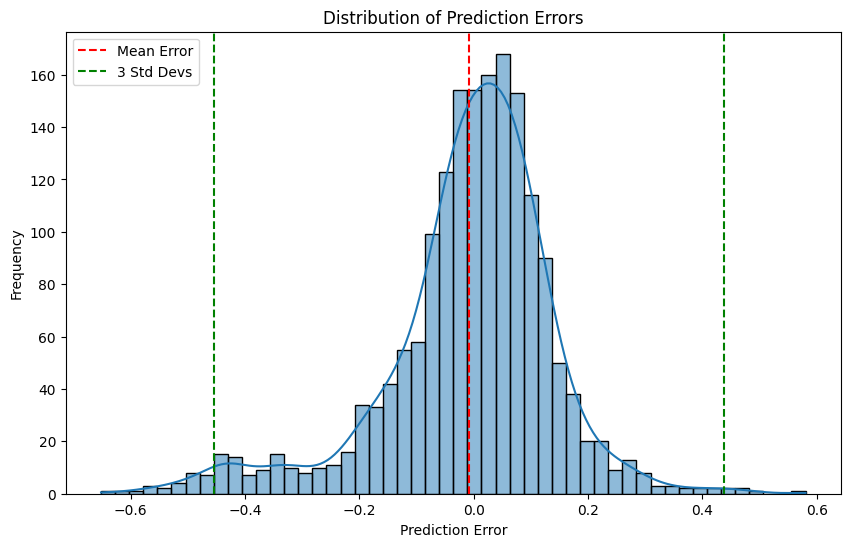
\includegraphics[width=\textwidth]{graphics/ErrorDistribution.png}
    \caption{Distributie van de voorspelfouten met de drempel voor anomaliedetectie \((\text{mean\_error} + 3 \cdot \text{std\_dev})\).}
    \label{fig:ErrorDistribution}
\end{figure}

\subsubsection{Evaluatieproces}
Het evaluatieproces omvat:
\begin{itemize}
    \item Het uitvoeren van het model op de testset en het berekenen van de bovengenoemde statistische maten.
    \item Het analyseren van de voorspellingsresultaten om te beoordelen hoe goed het model het werkelijke energieverbruik heeft voorspeld.
    \item Het gebruik van visualisaties zoals plots van voorspelde versus werkelijke waarden om visueel de prestaties en de afwijkingen te beoordelen.
\end{itemize}

\subsubsection{Conclusie van de Evaluatie}
De resultaten van deze uitgebreide evaluatie geven niet alleen inzicht in de prestaties van het model, maar stellen ArcelorMittal ook in staat om op data gebaseerde beslissingen te nemen over energiebeheer. Door continu de effectiviteit van het model te beoordelen en te verbeteren, kan het bedrijf de nauwkeurigheid van zijn energievoorspellingen verhogen en potentiële besparingen realiseren.



